% 03-experimental-setup-and-test-cases.tex
% ---------------------------

% Section Title
\section{EXPERIMENTAL SETUP AND TEST CASES} \label{sec:experimental-setup-and-test-cases}

    % Main Content

    \ldots

    \subsection{Equipment and Configuration} \label{subsec:equipment-and-configuration}

        In this section, we describe the hardware and software configuration used to perform our network performance measurements. Table~\ref{tab:equipment-summary} summarizes the main devices, their interfaces, and relevant specifications. 

        \begin{table}[ht]
            \small
            \centering
            \caption{Summary of Hardware and Network Configuration}
            \label{tab:equipment-summary}
            \begin{tabular}{@{}l p{0.78\columnwidth}@{}}
            \toprule
            \textbf{Device} & \textbf{Key Specifications} \\
            \midrule
            \textbf{PC1} 
                & Victus 16-s1005nl Notebook \newline
                  \textit{Operating System:} Ubuntu 24.04.2~LTS \newline
                  \textit{Ethernet Interface:} Realtek RTL8111/8168/8211/8411 \newline
                  \textit{Wireless Interface:} Realtek RTL8852BE (802.11ax) \\
            \midrule
            \textbf{PC2} 
                & Microsoft Surface Laptop Go~3 \newline
                  \textit{Operating System:} Ubuntu 24.10 \newline
                  \textit{Ethernet Interface:} via Anker PowerExpand+ USB-C Hub \newline
                  \textit{Wireless Interface:} Intel Alder Lake-P CNVi (802.11ax) \\
            \midrule
            \textbf{Router} 
                & Vodafone Power Station Wi-Fi~6 \newline
                  \textit{Ethernet Ports:} 4 $\times$ 1\,GbE ports \newline
                  \textit{Wi-Fi:} Dual-band 802.11ax (2.4\,GHz / 5\,GHz) \\
            \midrule
            \textbf{Cables} 
                & CAT.5E (up to 1\,Gbps) \\
            \bottomrule
            \end{tabular}
        \end{table}

        % \noindent
        % \textbf{PC1 (Victus 16-s1005nl).}
        % This notebook runs Ubuntu 24.04.2~LTS (codename \texttt{noble}). 
        % Its onboard Ethernet adapter is a Realtek \\ RTL8111/8168/8211/8411 controller, 
        % supporting up to 1\,Gbps. 
        % Wireless connectivity is provided by a Realtek RTL8852BE PCIe 802.11ax card.

        % This notebook runs Ubuntu~24.04.2\,LTS and has a Realtek RTL8111/8168/8211/8411 Gigabit Ethernet controller. Its wireless interface is a Realtek RTL8852BE PCIe 802.11ax card.

        % \medskip
        % \noindent
        % \textbf{PC2 (Surface Laptop Go~3).}
        % This device also runs Ubuntu, version 24.10 (codename \texttt{oracular}). 
        % It lacks a built-in Ethernet port, so a USB-C hub (ANKER PowerExpand+ 7-in-1) 
        % is used to provide a Gigabit Ethernet interface. 
        % For wireless, it has an Intel Alder Lake-P PCH CNVi card (802.11ax).

        % This device runs Ubuntu~24.10. It does not include a built-in Ethernet port, so a USB-C Anker PowerExpand+ hub is used to provide a Gigabit Ethernet interface. For wireless, it is equipped with an Intel Alder Lake-P CNVi Wi-Fi 6 adapter.

        % \medskip
        % \noindent
        % \textbf{Router (Vodafone Power Station Wi-Fi~6).}
        % All test traffic traverses a Vodafone Power Station Wi-Fi~6 router, 
        % which provides four Gigabit Ethernet ports and dual-band Wi-Fi~6 
        % (2.4\,GHz and 5\,GHz). 
        % In all wired scenarios, we connect via the router’s 1\,GbE ports 
        % using Category~5e cables.

        % All test traffic traverses a Vodafone Power Station Wi-Fi~6 router, which provides four 1\,GbE ports and dual-band 802.11ax wireless connectivity.

        % \medskip
        % \noindent
        % \textbf{Cables (CAT.5E).}
        % We use CAT.5E cables for all wired experiments, supporting 
        % up to 1\,Gbps throughput. 

        % We use Category~5E cables (rated for up to 1\,Gbps) for all wired experiments. 

        % \medskip
        This hardware setup allows us to compare Ethernet versus Wi-Fi performance 
        under a consistent router and cabling environment. 
        In the next section, we detail the evaluation scenarios and 
        the measurement methodology.

        % This setup allows for direct comparison of wired (Ethernet) versus wireless (Wi-Fi~6) performance under the same routing and cabling conditions. The next subsection details the test scenarios and configurations used in our experiments.

    \subsection{Evaluation Scenarios} \label{subsec:evaluation-scenarios}

        \ldots

        \begin{figure}[ht]
            \centering
            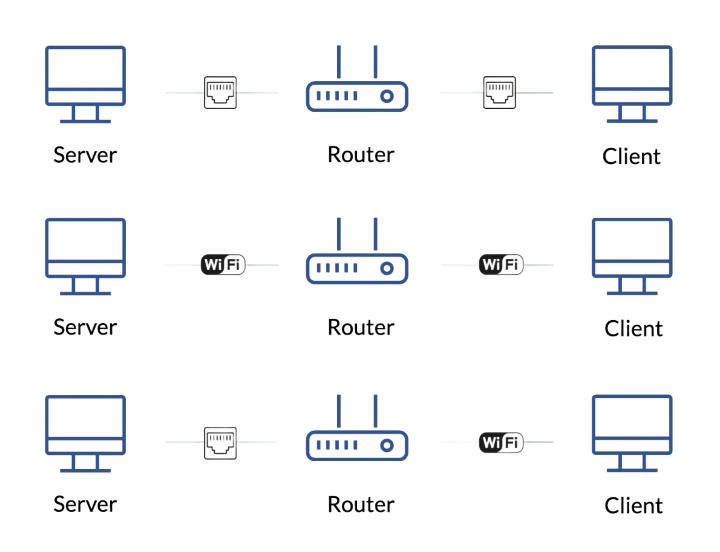
\includegraphics[width=0.8\columnwidth]{../images/test_cases_white.png}
            \caption{Test cases setup for the experiments.}
            \label{fig:test-cases}
        \end{figure}

        \ldots
